\documentclass[11pt]{article}
\usepackage[]{authblk}
\usepackage{graphicx}
\usepackage{color}
\usepackage{longtable}
\usepackage{hanging}
\usepackage{indentfirst}
\usepackage{setspace}
\usepackage{verbatim}
\usepackage{upgreek}
\usepackage{framed}
\usepackage{ textcomp }
\usepackage[weather]{ifsym}
\usepackage{natbib}
\usepackage{url}
\usepackage{soul}
\usepackage{amsmath, amsfonts,amssymb,mathrsfs}
\usepackage{fancyhdr}
\usepackage[compact]{titlesec}
\usepackage[T1]{fontenc}
\usepackage{lmodern}

\setlength{\evensidemargin}{0in}
\setlength{\headheight}{0in}
\setlength{\headsep}{0in}
\setlength{\oddsidemargin}{-0.25in}
\setlength{\paperheight}{11in}
\setlength{\paperwidth}{8.5in}
\setlength{\tabcolsep}{0in}
\setlength{\textheight}{9in}
\setlength{\textwidth}{7in}
\setlength{\topmargin}{0in}
\setlength{\topskip}{0in}
\setlength{\voffset}{0in}
%\setstretch{2}
%\raggedright
\parskip = 0.15in
\pagestyle{plain}
\setlength{\parindent}{0cm}

\definecolor{citescol}{RGB}{194,101,1}
%\definecolor{citescol}{RGB}{73,0,165}
\definecolor{urlscol}{RGB}{0,150,206}
%\definecolor{urlscol}{RGB}{0,107,124}
%\definecolor{linkscol}{RGB}{187,24,0}
\definecolor{linkscol}{RGB}{149,0,207}
%\definecolor{linkscol}{RGB}{73,0,165}
\definecolor{mycol}{RGB}{25,23,191}
\definecolor{outputcol}{RGB}{34,139,34}


%\def\Fld@bordercolor{1 0 0}
%\renewcommand*{\DefaultHeightofTextMultiline}{6\baselineskip} 
%\renewcommand*{\LayoutTextField}[2]{\makebox[6em][l]{#1 }%
%  \raisebox{\baselineskip}{\raisebox{-\height}{#2}}}
%\def\LayoutChoiceField#1#2{\makebox[6em][l]{#1 }#2}

%\LayoutTextField{label}{field}

\DeclareMathAlphabet{\msfsl}{T1}{cmr}{m}{it}
\DeclareMathAlphabet{\msyf}{OMX}{pcr}{m}{it}
\newcommand{\alf}{\upalpha}
\newcommand{\hilight}[1]{\colorbox{yellow}{#1}}

\newcommand{\levelone}[1]{
\bigskip
\noindent{\LARGE{\textsc{#1}}}
\vspace {0.05in}
}

\newcommand{\leveltwo}[1]{
\bigskip
\noindent{\Large{\textit{#1}}}
\vspace {-1mm}
}

\newcommand{\descriptionhead}[1]{
\noindent{\textbf{\textit{#1}}}\\ \vspace{-7mm}
}

\newcommand{\dhead}[1]{
\noindent{\textbf{\textit{#1 --}}}
}


\newcommand{\exs}[1]{
\vspace{-4mm}
\begin{itemize}
\item #1 \\ \vspace{-8mm}
\end{itemize}
}

\newcommand{\nbo}[1]{{\color{red}{#1}}}


\newcommand{\stepbullet}{\noindent \textbullet \ }
\newcommand{\mi}[1]{\textbf{\textit{#1}}}


\newcommand{\levelthree}[1]{\textit{#1 --}}

%\newcommand{\bowtiecirclefig}{{\rlap{\rlap{{\textbf{\BigCircle}}}{\FilledTriangleLeft}}\FilledTriangleRight}}

\bibliographystyle{bib_tex/mbe}
\bibpunct[; ]{(}{)}{;}{a}{,}{;}


\usepackage[breaklinks]{hyperref}
\usepackage[all]{hypcap}
\hypersetup{colorlinks=true,linkcolor=linkscol,citecolor=citescol,urlcolor=urlscol}


\usepackage{framed}
\usepackage[]{listings}
\usepackage{fontspec}
\usepackage{placeins}
\usepackage{epstopdf}

\lstset{breaklines=true}

\definecolor{shadecolor}{RGB}{238,224,229}


\setlength{\topmargin}{-0.4in}
\setlength{\headheight}{14.5pt}
\pagestyle{fancy}

\newcommand{\taha}[1]{{\textcolor{red}{[TAH comment: #1]}}} % TAH comment

\titlespacing{\section}{0pt}{*0}{*0}
\titlespacing{\subsection}{0pt}{*0}{*0}
\titlespacing{\subsubsection}{0pt}{*0}{*0}

\titleformat{\section}
  {\normalfont\Large\bfseries\color{mycol}}
  {\thesection}{1em}{}

\titleformat{\subsection}
  {\normalfont\large\bfseries\color{mycol}}
  {\thesubsection}{1em}{}

\titleformat{\subsubsection}
  {\normalfont\bfseries\color{mycol}}
  {\thesubsection}{1em}{}

% command for MrBayes command-line step
\newcommand{\cl}[1]{{\texttt{\textbf{#1}}}}

\newcommand{\colx}[1]{{\textcolor{tcol}{#1}}}

\newcommand{\mbcl}[1]{\exs{\cl{MrBayes > {#1}}}}

\newcommand{\rbprmt}{RevBayes > } 
\newcommand{\rbcl}[1]{\exs{\cl{\rbprmt{#1}}}}
\newcommand{\rbout}[1]{\exs{\cl{\textcolor{outputcol}{#1}}}}
\newcommand{\rbdn}{{\Large \symbol{126}}} % This makes a copy/pasteable tilde
\newcommand{\rbclml}[1]{\exs{\cl{\ \ \ \ \ \ \ \ \ \ \ {#1}}}}

% text box settings
% requires compiling w/ XeLaTeX
\newfontfamily\listingsfont[Scale=1.0]{Courier New}
\lstset{basicstyle=\listingsfont, columns=texcl}
\defaultfontfeatures{Mapping=tex-text}


\makeatletter
\lst@CCPutMacro\lst@ProcessOther {"2D}{\lst@ttfamily{-{}}{-{}}}
\@empty\z@\@empty
\makeatother

\begin{document}
\renewcommand{\headrulewidth}{0.5pt}
\headsep = 20pt
\lhead{ }
\rhead{\textsc {RevBayes Tutorial --- Substitution Models}}

\thispagestyle{plain}
\begin{center}

\textbf{\LARGE Phylogenetic Inference using RevBayes}\\\vspace{2mm}
\textbf{\it{\Large Substitution Models}}\\\vspace{2mm}
\end{center}

\section*{Overview}


This tutorial demonstrates how to set up and perform an analysis for different substitution models. 
You will create a phylogenetic model for the evolution of DNA sequences under a JC, HKY85, GTR, GTR+Gamma and GTR+Gamma+I substitution model.
For all these models you will perform an MCMC run to estimate phylogeny and other model parameters.

\subsection*{Requirements}
We assume that you have completed the following tutorials:
\begin{itemize}
\item RB\_Basics\_Tutorial
\end{itemize}



%
%\subsection*{Analysis Functions}
%
\newpage
\FloatBarrier
\section{Exercise: Character Evolution under various Substitution Models}

%\subsection{Introduction}
%
%
%\bigskip
%\section{Model Selection \& Partitioning using Bayes Factors}

For phylogenetic graphical model representations, \citet{hoehnaGM2014} introduced a new element called the \textit{tree plate}. 
This is a convenience for visualization because, although a phylogenetic tree is a graphical model, the complexity becomes intractable for large trees. 
Thus, the tree plate depicts replication over a given topology. 
The full graphical model with the unrooted tree plate for the GTR$+\Gamma$ model used in this tutorial is shown in Figure \ref{gtrgmfig}. Note that even unrooted analyses arbitrarily assign a root node to orient the tree.
\begin{figure}[h!]
\centering
\fbox{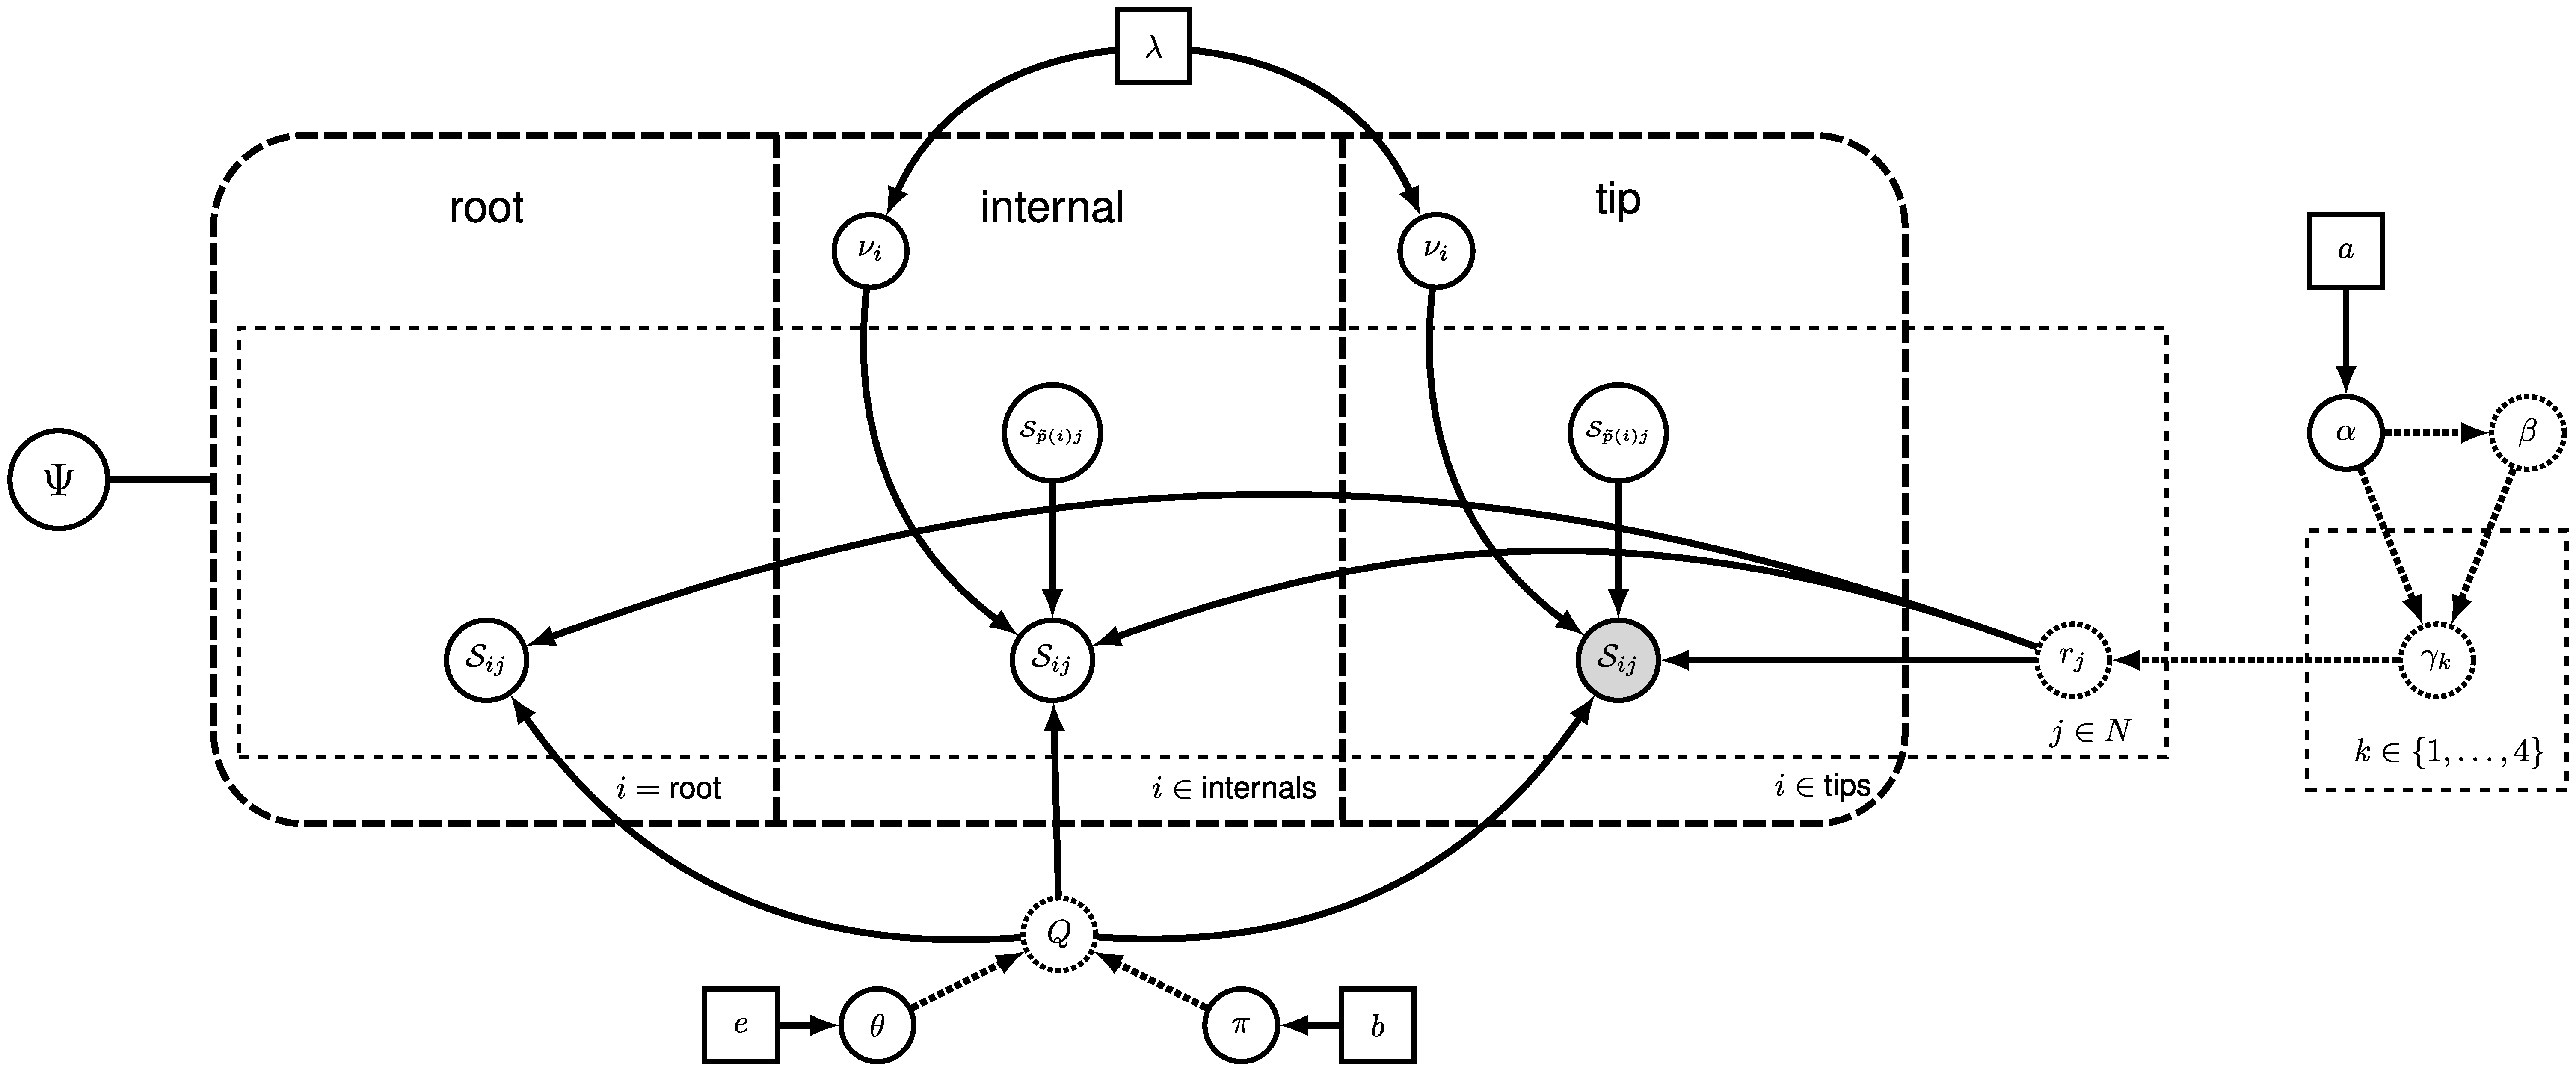
\includegraphics[width=6.8in,angle=0]{figures/gtrg_graphical_model}}
\caption{\small  The general-time reversible model \citep{tavare86} with gamma-distributed rate variation across sites \citep{yang94a}: GTR$+\Gamma$. 
The tree plate separates the nodes of the tree into different categories. For any tree there is a vector of tip nodes, a vector of internal nodes, and a root node. 
The stochastic node $\Psi$ orders the nodes in the tree plate. This representation allows for a simpler presentation of a complex model on a tree.
Each internal and tip node have a branch length applied to the branch connecting to the parent node. The branch length for node $i$ is denoted by the stochastic node $\nu_i$, and every branch-length node is conditioned on the rate parameter $\lambda$ of the exponential hyperprior.
The parameters of the GTR model include the exchangability rates $\theta$ and the equilibrium base frequencies $\pi$. 
The node $\theta$ is dependent on the constant hyperparameter $e$ which represents the vector of concentrations that control the Dirichlet prior on the stochastic node $\theta$.
Likewise, the stochastic node $\pi$ depends on the Dirichlet parameters specified in $b$.
The site rate model represented here is the discretized gamma model over four rate categories.
The stochastic node denoted $\alpha$ controls the shape of that gamma distribution.
The rate parameter $\beta$ of the gamma distribution is a deterministic node. Since we assume that the mean of the distribution on site rates is equal to $1$, then the function that determines the value of $\beta$ is $\beta = \alpha$.
The density of the gamma is discretized into 4 rate categories and the rate for each category is $\gamma_k$, for $k \in {1,\ldots,4}$. 
Then a rate value is computed for each site: $r_j$ for $j \in N$, where $N$ is the number of sites. 
}
\label{gtrgmfig}
\end{figure}

For any phylogenetic model using homologous characters, the state at the tips --- e.g., the nucleotide at a given position in the alignment --- is the observed value and clamped to the phylogenetic continuous-time Markov chain (CTMC). 
The state at any node is conditionally dependent on the sate of the parent node, thus knowing the topological ordering of nodes is important. 
Further, the state at any node is also dependent on other variables, such as the branch length, site rate, base frequencies, and relative substitution rates in a GTR$+\Gamma$ model as in Figure \ref{gtrgmfig}. 
This structure can be shown explicitly in a graphical model by fully representing the tree \citep[for examples see][]{hoehnaGM2014}.
However, even a relatively small tree of 15 tips becomes difficult to represent in this way. 
Thus, the tree plate shows this structure and can also depict the topology as a stochastic node (fig. \ref{gtrgmfig})



\bigskip
\subsection{Getting Started}

For the exercises outlined in this tutorial, we will use \RevBayes~interactively by typing commands in the command-line console.
The format of this exercise uses \colorbox{shadecolor}{\tt lavender blush shaded boxes} to delineate important steps. 
The various \RevBayes~commands and syntax are specified using \cl{typewriter text}. 
And the specific commands that you should type (or copy/paste) into \RevBayes~are indicated by shaded box and prompt. 
For example, after opening the \RevBayes~program, you can load your data file:

{\tt \begin{snugshade*}
\begin{lstlisting}
RevBayes > data_ITS <- readCharacterData("data/fagus_ITS.nex")
\end{lstlisting}
\end{snugshade*}}

For this command, type in the command and its options:\\ \cl{data\_ITS <- readCharacterData("data/fagus\_ITS.nex")}. 
\textbf{DO NOT} type in ``\cl{RevBayes >}'', the prompt is simply included to replicate what you see on your screen. 

This tutorial also includes hyperlinks: bibliographic citations are {\textcolor{citescol}{burnt orange}} and link to the full citation in the references, external URLs are {\textcolor{urlscol}{cerulean}}, and internal references to figures and equations are {\textcolor{linkscol}{purple}}.

The various exercises in this tutorial take you through the steps required to perform phylogenetic analyses of the example datasets. 
In addition, we have provided the output files for every exercise so you can verify your results. (Note that since the MCMC runs you perform will start from different random seeds, the output files resulting from your analyses \textit{will not} be identical to the ones we provide you.)

\exs{Download data and output files from:\\ \href{https://www.nescent.org/sites/academy/RevBayes\_Workshop\_Schedule}{https://www.nescent.org/sites/academy/RevBayes\_Workshop\_Schedule}
%\href{http://treethinkers.org/phylogenetic-inference-using-mrbayes-v3-2/}{\small link}
}


\exs{Open the file \cl{data/fagus\_ITS.nex} in your text editor. This file contains the sequences for the ITS gene sampled from 13 species (Box 1). The elements of the \cl{DATA} block indicate the type of data, number of taxa, and length of the sequences.}


\begin{center}
Box 1: A fragment of the NEXUS file containing the ITS sequences for this exercise. \\
\end{center}
{\tt \scriptsize \begin{framed}
\begin{lstlisting}
#NEXUS 

Begin data;
Dimensions ntax=13 nchar=673;
Format datatype=DNA missing=? gap=-;
Matrix
Trig_excelsa   
TCGAAACCTG...
Fagus_engleriana   
TCGAAACCTG...
Fagus_crenata1   
TCGAAACCTG...
Fagus_japonica2   
TCGAAACCTG...
Fagus_japonica1   
TCGAAACCTG...
Fagus_orientalis   
TCGAAACCTG...
Fagus_sylvatica   
TCGAAACCTG...
Fagus_lucida1   
TCGAAACCTG...
Fagus_lucida2   
TCGAAACCTG...
Fagus_crenata2   
TCGAAACCTG...
Fagus_grandifolia   
TCGAAACCTG...
Fagus_mexicana   
TCGAAACCTG...
Fagus_longipetiolata   
TCGAAACCTG...
	;
End;
\end{lstlisting}
\end{framed}}

\exs{Also note that ``pre-cooked'' output files are provided in the download. Throughout this tutorial, you can use those files to summarize output if you do not have time to run the full analyses yourself.}



\bigskip
\subsection{Launch RevBayes}

Execute the RevBayes binary. If this program is in your path, then you can simply type in your Unix terminal:

\exs{\cl{\$ rb}}

When you execute the program, you will see the program information, including the current version number and functions that will provide information about the program --- \cl{contributors()} and \cl{license()}. 




\bigskip
\subsection{An Unpartitioned Analysis}\label{secUnif} 

{\large \textcolor{mycol}{\textsc{Black Box Analysis}}}

This exercise involves 
\begin{enumerate}
\item setting up a sequence evolution model using
\begin{enumerate}
\item a Jukes-Cantor substitution process model,
\item an HKY substitution process model, 
\item a GTR substitution process model,
\item a GTR+$\Gamma$ substitution process model,
\item a GTR+$\Gamma$+I substitution process model,
\end{enumerate} 
\item approximating the posterior probability of the tree topology and branch lengths (and all other parameters) using MCMC,  
\item summarizing the MCMC output by computing the maximum a posteriori tree, and
\item estimating the marginal likelihood of the model using stepping-stone and path sampling. 
\end{enumerate}

All of the files for this analysis are provided for you and you can run these without significant effort using the \cl{source()} function in the \RevBayes~console:
{\tt \begin{snugshade*}
\begin{lstlisting}
RevBayes > source("RevBayes_scripts/full_analysis.Rev")
\end{lstlisting}
\end{snugshade*}}

If everything loaded properly, then you should see the program begin running the posterior analysis needed for estimating the posterior probabilities. If you continue to let this run, then you will see it output the states of the Markov chain once the MCMC analysis begins.

Ultimately, this is how you will execute most analyses in \RevBayes~and the full specification of the model and analyses are contained in the sourced files. 
You could easily run this entire analysis on your own data if you changed the name of the files containing the tutorial's sequences in one of the model specification files, e.g.: \cl{RB\_tutorial\_files/models/noclock\_GTR\_model.Rev}. 
However, it is important to understand the components of the model to be able to take advantage of the flexibility and richness of \RevBayes.
Furthermore, without inspecting the \Rev~scripts sourced in \cl{full\_analysis.Rev}, you may have inadvertently conducted an inappropriate analysis on your dataset, which would be a waste of your time and CPU cycles. 
The next steps will walk you through the full specification of the model and MCMC analyses. 

\bigskip
{\large \textcolor{mycol}{\textsc{Full Model Specification}}}

\textbf{\textit{Load Data}}

First load in the sequences using the \cl{readCharacterData()} function. This function returns a \textit{single} data matrix or a \textit{vector} of data matrices depending on how many matrices there are in the data file. (You will also note that list indexing in Rev starts with \cl{1} like in the R language.)
{\tt \begin{snugshade*}
\begin{lstlisting}
RevBayes > data_ITS <- readCharacterData("data/fagus_ITS.nex")
RevBayes > data_rbcL <- readCharacterData("data/fagus_rbcL.nex")
RevBayes > data_matK <- readCharacterData("data/fagus_matK.nex")
\end{lstlisting}
\end{snugshade*}}
Executing these lines initializes each data matrix as their respective \Rev~variables. 
This exercise assumes a single model for all three genes and thus we need to combine the three datasets.
Concatenate the three data matrices using the \cl{+} operator. 
This returns a single data matrix with all genes.

{\tt \begin{snugshade*}
\begin{lstlisting}
RevBayes > data <- data_ITS + data_rbcL + data_matK
\end{lstlisting}
\end{snugshade*}}

To report the current value of any variable, simply type the variable name and press enter. 
For the \cl{data} matrix, this provides information about the alignment:

{\tt \begin{snugshade*}
\begin{lstlisting}
RevBayes > data
   DNA character matrix with 13 taxa and 2576 characters
   =====================================================
   Origination:                   fagus_ITS.nex
   Number of taxa:                13
   Number of characters:          2576
   Number of included characters: 2576
   Datatype:                      DNA
\end{lstlisting}
\end{snugshade*}}


Next we will specify some useful variables based on our dataset. 
The variable \cl{data} has \textit{member functions} that we can use to retrieve information about the dataset. 
These include the number of species (\cl{n\_species}), the tip labels (\cl{names}), and the number of internal branches (\cl{n\_branches}).
Each of these variables will be necessary for setting up different parts of our model.
{\tt \begin{snugshade*}
\begin{lstlisting}
RevBayes > n_species <- data.ntaxa()
RevBayes > names <- data.names()	
RevBayes > n_branches <- 2 * n_species - 3 
\end{lstlisting}
\end{snugshade*}}

Now we can proceed with building our different substitution models.

\subsection*{Substitution process models}

In the subsection following below we will describe and give example \Rev~code for different substitution models. 
In all the analyses the remaining parts of the model and analysis remain the same.
Thus, to safe some space in this tutorial we will only present once how to set up the distribution on trees, perform the MCMC algorithm and analyze the data.
You should create and run models for each of the substitution processes independently.
You can find example \Rev~scripts in the directory of this tutorial.

\subsubsection*{Jukes-Cantor (JC)  substitution process model}

The Jukes-Cantor (JC) substitution model is the simplest substitution model.
It does not need any additional parameters because all the base frequencies and the exchangeability rates are equivalent.
The only parameter that we need to give the \cl{JC} function is the number of states, which is 4 in our example.
We could also have used a JC substitution model with 20 states if our data were amino acid sequences.
In general, any number of states can be used for the JC substitution model.
Note that the number of states will not be a part of the model graph because it only defines the type of \cl{JC} function.
We also do not need a deterministic variable for the rate matrix and instead a constant variable suffices. 
{\tt \begin{snugshade*}
\begin{lstlisting}
RevBayes > Q <- JC(4)
\end{lstlisting}
\end{snugshade*}}


\subsubsection*{Hasegawa-Kishino-Yano (HKY)  substitution process model}


First, we will define and specify a prior on the base frequencies rates of the HKY model. 
We will use a flat Dirichlet prior distribution on these four frequencies. 
To do this, we must begin by defining a constant node that specifies the vector of concentration values of the Dirichlet prior using the \cl{v()} function:
{\tt \begin{snugshade*}
\begin{lstlisting}
RevBayes > pi_prior <- v(1,1,1,1) 
\end{lstlisting}
\end{snugshade*}}


The constant node \cl{pi\_prior} corresponds to the node labeled $b$ in the graphical model depicted in Figure \ref{gtrgmfig}. 
The vector function, \cl{v()}, creates a vector of six values. 
Display the current value of \cl{pi\_prior} by simply typing the variable name:
{\tt \begin{snugshade*}
\begin{lstlisting}
RevBayes > pi_prior
       [ 1, 1, 1, 1 ]
\end{lstlisting}
\end{snugshade*}}
This node defines the parameters of the Dirichlet prior distribution on the base frequencies.
Thus, we can create a stochastic node for the base frequencies using the \cl{dnDirichlet()} function, which takes a vector of values as an argument and the \cl{\rbdn} operator. 
Together, these create a stochastic node named \cl{er} ($\pi$ in Figure \ref{gtrgmfig}): 
{\tt \begin{snugshade*}
\begin{lstlisting}
RevBayes > pi ~ dnDirichlet(pi_prior)
\end{lstlisting}
\end{snugshade*}}


The Dirichlet distribution assigns probability densities to grouped parameters: {\it e.g.}, those that measure proportions and must sum to 1. 
Above, we specified a 4-parameter Dirichlet prior on the base frequencies of the HKY model, where the placement of each value specified represents one of the 4 frequencies: 
(1) $\pi_A$, 
(2) $\pi_C$, 
(3) $\pi_G$, 
(4) $\pi_T$.
The input parameters of a Dirichlet distribution are called shape parameters or concentration parameters and a value is specified for each of the 4 HKY frequencies. 
The expectation and variance for each variable are related to the sum of the shape parameters.
The prior above is a `flat' or symmetric Dirichlet since all of the shape parameters are equal (1,1,1,1), thus we are specifying a model that allows for equal frequencies of nucleotides, such that the expected rate for each is equal to $\frac{1}{4}$ \citep{zwickl04}.
Figure \ref{dirichletFig}a shows the probability density of each frequency under this model.
If we parameterized the Dirichlet distribution such that all of the parameters were equal to 100, this would also specify a prior with an expectation of equal base frequencies (Figure \ref{dirichletFig}b). 
However, by increasing the shape parameters of the Dirichlet distribution, \cl{pi\_prior <- v(100,100,100,100)}, would heavily restrict the MCMC from sampling sets of HKY frequencies in which the values were not equal or very nearly equal ({\it i.e.}, this is a very {\em informative} prior). 
We can consider a different Dirichlet parameterization if we had strong prior belief that the GC content is very high.
In this case, we could specify a more informative prior density: \cl{pi\_prior <- v(4,8,8,4)}. 
Under this model, the expected GC frequency would be $\frac{16}{24}$ (Figure \ref{dirichletFig}c). 
An alternative informative prior would be one where we assumed that each of the 4 HKY frequencies had a different value conforming to a Dirichlet(2,4,6,8). 
This would lead to a different prior probability density for each rate parameter (Figure \ref{dirichletFig}d).
Without strong prior knowledge about the pattern of base frequencies, however, we can better capture our statistical uncertainty with a vague prior on the HKY base frequencies. 
Notably, all patterns of base frequencies have the same probability density under \cl{pi\_prior <- v(1,1,1,1)}.
\begin{figure}[h!]
\centering
\fbox{\includegraphics[width=5in,angle=-90]{figures/dirichlet_rates.eps}}
\caption{\small Four different examples of Dirichlet priors on exchangeability rates.}
\label{dirichletFig}
\end{figure}

For each stochastic node in our model, we must also specify a proposal mechanism if we wish to sample that value. 
The Dirichlet prior on our parameter \cl{pi} creates a \href{http://en.wikipedia.org/wiki/Simplex}{\textit{simplex}} of values that sum to 1. 
In \RevBayes, there are many different proposal mechanisms -- called \textit{moves} -- and each move operates on a specific data type (called RevType). 
Check the RevType of the variable \cl{pi} using the \cl{structure()} function:
{\tt \small \begin{snugshade*}
\begin{lstlisting}
RevBayes > structure(pi)

   _variable     = pi <0x7fc5b1e08000>
   _RevType      = Simplex
   _RevTypeSpec  = [ Simplex, Container, RevObject ]
   _value        = [ 0.124413, 0.812981, 0.0150606, 0.0475456 ]
   _size         = 4
   _dagNode      = pi <0x7fc5b1e07290>
   _dagType      = Stochastic DAG node
   _refCount     = 1
   _distribution = <0x7fc5b1e079f0>
   _touched      = TRUE
   _clamped      = FALSE
   _lnProb       = -inf
   _storedLnProb = 1.25594e-308
   _parents      = [ pi_prior <0x7fc5b1e07e60> ]
   _children     = [  ]
\end{lstlisting}
\end{snugshade*}}

The \cl{structure()} function -- which has an accepted abbreviation of \cl{str()} -- is verbose and provides a lot of information that may at first appear confusing. 
Much of this information is helpful primarily for troubleshooting and debugging purposes, however, the components that you may want to look at are: \cl{RevType}, \cl{value}, \cl{dagType}, \cl{clamped}, \cl{lnProb}, and the names of the \cl{variable}, \cl{parents}, and \cl{children}.

We must create a vector containing all of the moves for each of our stochastic nodes. 
This vector will be passed in to the function constructing our MCMC or power posterior runs.
All moves in the Rev language are called \cl{mv*}, where \cl{*} is a wild card for the move name. 
Initialize the first element of our vector of moves by setting the proposal on the base frequencies:

{\tt\small \begin{snugshade*}
\begin{lstlisting}
RevBayes > moves[1] <- mvSimplexElementScale(pi) 
\end{lstlisting}
\end{snugshade*}}


The various proposal mechanisms available in \RevBayes~each require specific input arguments. 
The \cl{mvSimplexElementScale} move can only operate on a simplex and the first argument is the stochastic node that you wish to update. 


The second parameter of the HKY model is the transition-transversion rate, \cl{kappa}.
For the transition transversion rate we choose a lognormal prior distribution.
{\tt\small \begin{snugshade*}
\begin{lstlisting}
kappa ~ dnLnorm(1.0,1.25)
\end{lstlisting}
\end{snugshade*}}

Again, we need to add move changing the transition-transversion rate during the MCMC.
We choose here a simple scaling proposal.
{\tt\small \begin{snugshade*}
\begin{lstlisting}
RevBayes > moves[2] <- mvScale(kappa) 
\end{lstlisting}
\end{snugshade*}}


We can finish setting up this part of the model by creating a deterministic node for the HKY rate matrix \cl{Q}. 
The \cl{hky()} function takes a transition-transversion rate and a set of base frequencies to compute the rate matrix used when calculating the likelihood of our model.
{\tt \begin{snugshade*}
\begin{lstlisting}
RevBayes > Q := hky(kappa,pi)
\end{lstlisting}
\end{snugshade*}}



\subsubsection*{General Time Reversible (GTR) substitution process model}

First, we replicate the prior distribution and creation of the base frequency variable.
{\tt\small \begin{snugshade*}
\begin{lstlisting}
RevBayes > pi_prior <- v(1,1,1,1) 
RevBayes > pi ~ dnDirichlet(pi_prior)
RevBayes > moves[1] <- mvSimplexElementScale(pi) 
\end{lstlisting}
\end{snugshade*}}

Then, we will define and specify a flat prior on the exchangeability rates of the GTR model. 
{\tt \begin{snugshade*}
\begin{lstlisting}
RevBayes > er_prior <- v(1,1,1,1,1,1) 
\end{lstlisting}
\end{snugshade*}}

This node defines the parameters of the Dirichlet prior distribution on the exchangeability rates.
Thus, we can create a stochastic node for the exchangeability rates using the \cl{dnDirichlet()} function. 
Together, these create a stochastic node named \cl{er} ($\theta$ in Figure \ref{gtrgmfig}): 
{\tt \begin{snugshade*}
\begin{lstlisting}
RevBayes > er ~ dnDirichlet(er_prior)
\end{lstlisting}
\end{snugshade*}}


We specified a 6-parameter Dirichlet prior on the relative rates of the GTR model, where the placement of each value specified represents one of the 6 relative rates: 
(1) $A\leftrightarrows C$, 
(2) $A\leftrightarrows G$, 
(3) $A\leftrightarrows T$, 
(4) $C\leftrightarrows G$, 
(5) $C\leftrightarrows T$, 
(6) $G\leftrightarrows T$. 


Then, we create the same simplex move as for the base frequencies.
{\tt\small \begin{snugshade*}
\begin{lstlisting}
RevBayes > moves[2] <- mvSimplexElementScale(er) 
\end{lstlisting}
\end{snugshade*}}



We finish setting up this part of the model by creating a deterministic node for the GTR rate matrix \cl{Q}. 
The \cl{gtr()} function takes a set of exchangeability rates and a set of base frequencies to compute the rate matrix used when calculating the likelihood of our model.
{\tt \begin{snugshade*}
\begin{lstlisting}
RevBayes > Q := gtr(er,pi)
\end{lstlisting}
\end{snugshade*}}


\subsection*{Gamma-Distributed Site Rates}


We will also assume that the substitution rates vary among sites according to a gamma distribution, which has two parameters: the shape parameter, $\alpha$, and the rate parameter, $\beta$. 
In order that we can interpret the branch lengths as the expected number of substitutions per site, this model assumes that the mean site rate is equal to 1.
The mean of the gamma is equal to $\alpha/\beta$, so a mean-one gamma is specified by setting the two parameters to be equal, $\alpha=\beta$.
Therefore, we need only consider the single shape parameter, $\alpha$ \citep{yang94a}. 
The degree of among-site substitution rate variation (ASRV) is inversely proportional to the value of the shape parameter---as the value of $\alpha$-shape parameter increases, the gamma distribution increasingly resembles a normal distribution with decreasing variance, which corresponds to decreasing levels of ASRV (Figure \ref{asrhGammaFig}).
If $\alpha = 1$, then the gamma distribution collapses to an exponential distribution with a rate parameter equal to $\beta$.
By contrast, when the value of the $\alpha$-shape parameter is $< 1$, the gamma distribution assumes a concave distribution that places most of the prior density on low rates but allows some prior mass on sites with very high rates, which corresponds to high levels of ASRV (Figure \ref{asrhGammaFig}).

\begin{figure}[h]
\centering
\fbox{\includegraphics[width=2.5in,angle=-90]{figures/asrh_gamma.eps}}
\caption{\small The probability density of mean-one gamma-distributed rates under different shape parameters.}
\label{asrhGammaFig}
\end{figure}


Alternatively, we might not have good prior knowledge about the variance in site rates, thus we can place an uninformative, or diffuse prior on the shape parameter.
For this analysis, we will use an exponential distribution with a rate parameter, \cl{shape\_prior}, equal to \cl{0.05}.
Under an exponential prior, we are placing non-zero probability on values of $\alpha$ ranging from 0 to $\infty$. 
The rate parameter, often denoted $\lambda$, of an exponential distribution controls both the mean and variance of this prior such that the expected (or mean) value of $\alpha$ is:
$\mathbb{E}[\alpha] = \frac{1}{\lambda}.$
Thus, if we set $\lambda=0.05$, then $\mathbb{E}[\alpha] = 20$.

Create a constant node called \cl{shape\_prior} for the rate parameter of the exponential prior on the gamma-shape parameter
{\tt\begin{snugshade*}
\begin{lstlisting}
RevBayes > shape_prior <- 0.05                                                                             
\end{lstlisting}
\end{snugshade*}}

Then create a stochastic node called \cl{shape} to represent the $\alpha$ node in Figure \ref{gtrgmfig}, with an exponential density as a prior:
{\tt\begin{snugshade*}
\begin{lstlisting}
RevBayes > shape ~ dnExponential(shape_prior)

\end{lstlisting}
\end{snugshade*}}

The way the ASRV model is implemented involves discretizing the mean-one gamma distribution into a set number of rate categories. 
Thus, we can analytically marginalize over the uncertainty in the rate at each site. 
To do this, we need a deterministic node that is a vector of rates calculated from the gamma distribution and the number of rate categories. 
The \cl{discretizeGamma()} function returns this deterministic node and takes three arguments: the shape and rate of the gamma distribution and the number of categories. Since we want to discretize a mean-one gamma distribution, we can pass in \cl{shape} for both the shape and rate.

Initialize the \cl{gamma\_rates} deterministic node vector using the  \cl{discretizeGamma()} function with \cl{4} bins:
{\tt \begin{snugshade*}
\begin{lstlisting}
RevBayes > gamma_rates := discretizeGamma( shape, shape, 4 )
\end{lstlisting}
\end{snugshade*}}



The random variable that controls the rate variation is the stochastic node \cl{shape}. This variable is a single, real positive value (\cl{RevType = RealPos}). 
We will apply a simple scale move to this parameter.
The scale move's tuning parameter is called \cl{lambda} and this value dictates the size of the proposal.
{\tt \begin{snugshade*}
\begin{lstlisting}
moves[3] <- mvScale(shape)\end{lstlisting}
\end{snugshade*}}


\subsection*{A model for invariant sites}

Under the invariant site model, every site of our sequence has the chance \cl{pinvar} to be invariant.
That mean, with probability \cl{pinvar} we do not observe any change along the phylogeny.
Here we specify a \cl{beta(1,1)} prior distribution on \cl{pinvar}.
The \cl{beta(1,1)} is equivalent to a uniform distribution, but has the nice advantage in \Rev~that a random variable from a beta distribution is of type \textit{Probability}.
{\tt \begin{snugshade*}
\begin{lstlisting}
RevBayes > pinvar ~ beta(1,1)
\end{lstlisting}
\end{snugshade*}}

We can also apply two different moves to the probability of a site being invariant:
{\tt \begin{snugshade*}
\begin{lstlisting}
RevBayes > moves[4] <- mvScale(pinvar)
RevBayes > moves[5] <- mvSlide(pinvar)
\end{lstlisting}
\end{snugshade*}}

\subsection*{Tree Topology and Branch Lengths}

The tree topology and branch lengths are also stochastic nodes in our model. 
In Figure \ref{gtrgmfig}, the tree topology is denoted $\Psi$ and the length of the branch leading to node $i$ is $\nu_i$.

We will assume that all possible labeled, unrooted tree topologies have equal probability. This is the \cl{dnUniformTopology()} distribution in RevBayes. Specify the \cl{topology} stochastic node by passing in the number of species \cl{n\_species} and tip labels \cl{names} to the \cl{dnUniformTopology()} distribution:
{\tt \begin{snugshade*}
\begin{lstlisting}
RevBayes > topology ~ dnUniformTopology(n_species, names)
\end{lstlisting}
\end{snugshade*}}

For some types of stochastic nodes there are several available moves. 
Often the different moves explore parameter space in a different way and nothing prevents one from using multiple different moves to improve mixing. 
For the unrooted tree topology, we can use both a nearest-neighbor interchange move (\cl{mvNNI}) and a subtree-prune and regrafting move (\cl{mvSPR}). These moves do not have tuning parameters associated with them, thus you only need to pass in the \cl{topology} node and \cl{weight} 
{\tt \begin{snugshade*}
\begin{lstlisting}
RevBayes > moves[6] <- mvNNI(topology)
RevBayes > moves[7] <- mvSPR(topology)
\end{lstlisting}
\end{snugshade*}}


Next we have to create a stochastic node for each of the $2N-3$ branches in our tree (where $N=$ \cl{n\_species}). 
We can do this using a \cl{for} loop --- this is a plate in our graphical model. In this loop, we can create each branch-length node and assign each move. Copy this entire block of \Rev~code into the console:
{\tt \small \begin{snugshade*}
\begin{lstlisting}
mi <- 7
for (i in 1:n_branches) {
   br_lens[i] ~ dnExponential(10.0)
   moves[mi++] <- mvScale(br_lens[i]) 
}
\end{lstlisting}
\end{snugshade*}}

It is convenient to monitor a deterministic variable of the branch lengths. In \MrBayes, \textit{tree length} was reported to the log file instead of the length of each branch. The tree length is the sum of all branch lengths and this can be computed using the \cl{sum()} function which calculates the sum of any vector of values.
{\tt \begin{snugshade*}
\begin{lstlisting}
RevBayes > tree_length := sum(br_lens)
\end{lstlisting}
\end{snugshade*}}

Finally, we can create a branch-length phylogeny by combining the tree topology and branch lengths using the \cl{treeAssembly()} function, which applies the value of the $i^{th}$ member of the \cl{br\_lens} vector to the branch leading to the $i^{th}$ node in \cl{topology}. Thus, the \cl{phylogeny} variable is a deterministic node: 

{\tt \begin{snugshade*}
\begin{lstlisting}
RevBayes > phylogeny := treeAssembly(topology, br_lens)
\end{lstlisting}
\end{snugshade*}}



\textbf{\textit{Putting it All Together}}

Now that we have initialized virtually all of our model parameters and we can link all of the parts in the stochastic node that will be clamped by the data. 
The sequence substitution model is a distribution called the \textit{phylogenetic continuous-time Markov chain} and we use the \cl{dnPhyloCTMC} constructor function to create this node.
This distribution requires several input arguments: (1) the \cl{tree} with branch lengths, (2) the instantaneous rate matrix \cl{Q}, the node characterizing the rate variation across sites (though \cl{siteRates} can be omitted if you do not assume rate variation across sites), (3) the probability of a site being invariant, and (4) the \cl{type} of character data.
{\tt \begin{snugshade*}
\begin{lstlisting}
RevBayes > phyloSeq ~ dnPhyloCTMC(tree=phylogeny, Q=Q, siteRates=gamma_rates, pInv=pinvar, type="DNA")
\end{lstlisting}
\end{snugshade*}}


Once the character evolution model has been created, we can attach our sequence data to the tip nodes in the tree.
{\tt \begin{snugshade*}
\begin{lstlisting}
RevBayes > phyloSeq.clamp(data)
\end{lstlisting}
\end{snugshade*}}
When this function is called, \RevBayes~sets each of the stochastic nodes representing the tip nodes of the tree to the sequence corresponding to that species in the alignment. 
This essentially tells the program that this is where the DAG ends and the states of the tip nodes are fixed. 

Now we can wrap up the whole model to conveniently access the DAG. To do this, we only need to give the \cl{model()} function a single node. With this node, the \cl{model()} function can find all of the other nodes by following the arrows in the graphical model:
{\tt \begin{snugshade*}
\begin{lstlisting}
RevBayes > mymodel <- model(topology)
\end{lstlisting}
\end{snugshade*}}

Now we have specified a simple, single-partition analysis---each parameter of the model will be estimated from every site in our alignment.
If we inspect the contents of \cl{mymodel} we can review all of the nodes in the DAG:
{\tt \begin{snugshade*}
\begin{lstlisting}
RevBayes > mymodel
\end{lstlisting}
\end{snugshade*}}

\bigskip
{\large \textcolor{mycol}{\textsc{Perform MCMC Analysis Under the GTR+Gamma+I Model}}}

This section will cover setting up the MCMC sampler and summarizing the posterior distribution of trees. 

\textbf{\textit{Specify Monitors}}

For our MCMC analysis we need to set up a vector of \textit{monitors} to save the states of our Markov chain. 
The monitor functions are all called \cl{mn*}, where \cl{*} is the wildcard representing the monitor type.
First, we will initialize the model monitor using the \cl{mnModel} function. This creates a new monitor variable that will output the states for all model parameters when passed into a MCMC function. 
{\tt \begin{snugshade*}
\begin{lstlisting}
RevBayes > monitors[1] <- mnModel(filename="output/fagus_noclock_GTR_Gamma_pInv_posterior.log", printgen=100)
\end{lstlisting}
\end{snugshade*}}

The \cl{mnFile} monitor will record the states for only the parameters passed in as arguments. We use this monitor to specify the output for our sampled trees and branch lengths.

{\tt \begin{snugshade*}
\begin{lstlisting}
RevBayes > monitors[2] <- mnFile(filename="output/fagus_noclock_GTR_Gamma_pInv_posterior.trees",printgen=100, phylogeny)
\end{lstlisting}
\end{snugshade*}}


Finally, create a screen monitor that will report the states of specified variables to the screen with \cl{mnScreen}:
{\tt \begin{snugshade*}
\begin{lstlisting}
RevBayes > monitors[3] <- mnScreen(printgen=10,  TL)
\end{lstlisting}
\end{snugshade*}}

\textbf{\textit{Initialize and Run MCMC}}

With a fully specified model, a set of monitors, and a set of moves, we can now set up the MCMC algorithm that will sample parameter values in proportion to their posterior probability. The \cl{mcmc()} function will create our MCMC object:
{\tt \begin{snugshade*}
\begin{lstlisting}
RevBayes > mymcmc <- mcmc(mymodel, monitors, moves)
\end{lstlisting}
\end{snugshade*}}


Now, run the MCMC:
{\tt \begin{snugshade*}
\begin{lstlisting}
RevBayes > mymcmc.run(generations=30000)
\end{lstlisting}
\end{snugshade*}}

When the analysis is complete, you will have the monitor files in your output directory.


\textbf{\textit{Summarize the MCMC Output}}

Methods for visualizing the marginal densities of parameter values are not currently available in \RevBayes. Thus, it is important to use programs like Tracer \citep{rambaut09} to evaluate mixing and non-convergence. (\RevBayes~does, however, have a tool for convergence assessment called \cl{beca}.)

\RevBayes~can also summarize the tree samples by reading in the tree-trace file:
{\tt \begin{snugshade*}
\begin{lstlisting}
RevBayes > treetrace <- readTreeTrace("output/fagus_noclock_GTR_Gamma_pInv_posterior.trees")
RevBayes > treetrace.summarize()
\end{lstlisting}
\end{snugshade*}}


The \cl{mapTree()} function will summarize the tree samples and write the maximum a posteriori tree to file:
{\tt \begin{snugshade*}
\begin{lstlisting}
RevBayes > mapTree(treetrace,"output/fagus_noclock_GTR_Gamma_pInv_map.tre")
\end{lstlisting}
\end{snugshade*}}





\bigskip
\subsection*{Batch Mode}

If you wish to run this exercise in batch mode, the files are provided for you. 

You can carry out these batch commands by providing the file name when you execute the \cl{rb} binary in your unix terminal (this will overwrite all of your existing run files).
\exs{\cl{\$ rb full\_analysis.Rev}}

\bigskip
\section*{Useful Links}

\begin{itemize}
\item RevBayes: \href{https://github.com/revbayes/code}{https://github.com/revbayes/code} \\ \vspace{-7mm}
\item MrBayes: \href{http://mrbayes.sourceforge.net/}{http://mrbayes.sourceforge.net} \\ \vspace{-7mm}
\item PhyloBayes: \href{http://megasun.bch.umontreal.ca/People/lartillot/www/index.htm}{http://www.phylobayes.org} \\ \vspace{-7mm}
\item Bali-Phy: \href{http://www.bali-phy.org/}{http://www.bali-phy.org} \\ \vspace{-7mm}
%\item BEAGLE: \href{http://code.google.com/p/beagle-lib/}{http://code.google.com/p/beagle-lib/} \\ \vspace{-7mm}
\item Tree Thinkers: \href{http://treethinkers.org/}{http://treethinkers.org} \\ \vspace{-7mm}
\end{itemize}

Questions about this tutorial can be directed to: \\\vspace{-10mm}
\begin{itemize}
\item Tracy Heath (email: \href{mailto:tracyh@berkeley.edu}{tracyh@berkeley.edu}) \\\vspace{-8mm}
\item Michael Landis (email: \href{mailto:mlandis@berkeley.edu}{mlandis@berkeley.edu}) \\\vspace{-8mm} 
\item Sebastian H\"{o}hna (email: \href{mailto:sebastian.hoehna@gmail.com}{sebastian.hoehna@gmail.com})
\\\vspace{-8mm} 
\item Brian R. Moore (email: \href{mailto:brianmoore@ucdavis.edu}{brianmoore@ucdavis.edu}) \\\vspace{-8mm}
\end{itemize}

\href{http://creativecommons.org/licenses/by/4.0/}{
\includegraphics[scale=0.8]{figures/ccby.eps}} This tutorial was written by \href{http://phylo.bio.ku.edu/content/tracy-heath}{Tracy Heath}, \href{http://michaeljameslandis.com/}{Michael Landis}, and Sebastian H\"{o}hna; licensed under a \href{http://creativecommons.org/licenses/by/4.0/}{Creative Commons Attribution 4.0 International License}. 
(This tutorial is based on the \href{http://treethinkers.org/tutorials/phylogenetic-inference-using-mrbayes-v3-2/}{Phylogenetic Inference using MrBayes v3.2} tutorial written by Tracy Heath, Conor Meehan, and Brian Moore and some content is reproduced here.
Mark Holder, Ben Liebeskind, Emily McTavish, and April Wright provided helpful comments.)

Version dated: \today

\nocite{sukumaran10,rannala96,robert02,rodrigue08,ronquist09,Rubinstein1981,simon01,Smith1993,Suchard2005,verdinelli95,wong08,Yang2007,Yang2005,yang97b}
%\newpage

%%%%%%%%%%%%%%%%%%%%%%%%%%%%%%%%%%%%
%  REFERENCES  
%%%%%%%%%%%%%%%%%%%%%%%%%%%%%%%%%%%%

{\renewcommand{\bibsection}{\section*{Relevant References}}


\bibliography{bib_tex/master_refs}




\end{document}
